\subsection{Sample and prevalence}
Of 1,741,240 original records, 24,895 met the STEM and employment eligibility criteria; 370 were excluded under the occupational rule (311 excluded-group and 59 military records). The analytical sample comprised 24,525 person-period records: 14,478 for training, 4946 for validation and 5101 for testing. In 2021, 4163 of 4792 evaluable records had an exact degree code; the remaining 629 could be assigned only to a compatible educational grouping. From 2022 onwards all evaluable records had exact degree codes.

Weighted mismatch varied between 35.64\% and 41.07\% (Figure~\ref{fig:annual}). In 2025, 1980 of 5101 records were classified as mismatched (unweighted 38.82\%); the weighted estimate was 40.28\% (approximate 95\% bootstrap interval 36.70--44.63\%). The series does not establish a monotonic trend.
\begin{figure}[htbp]\centering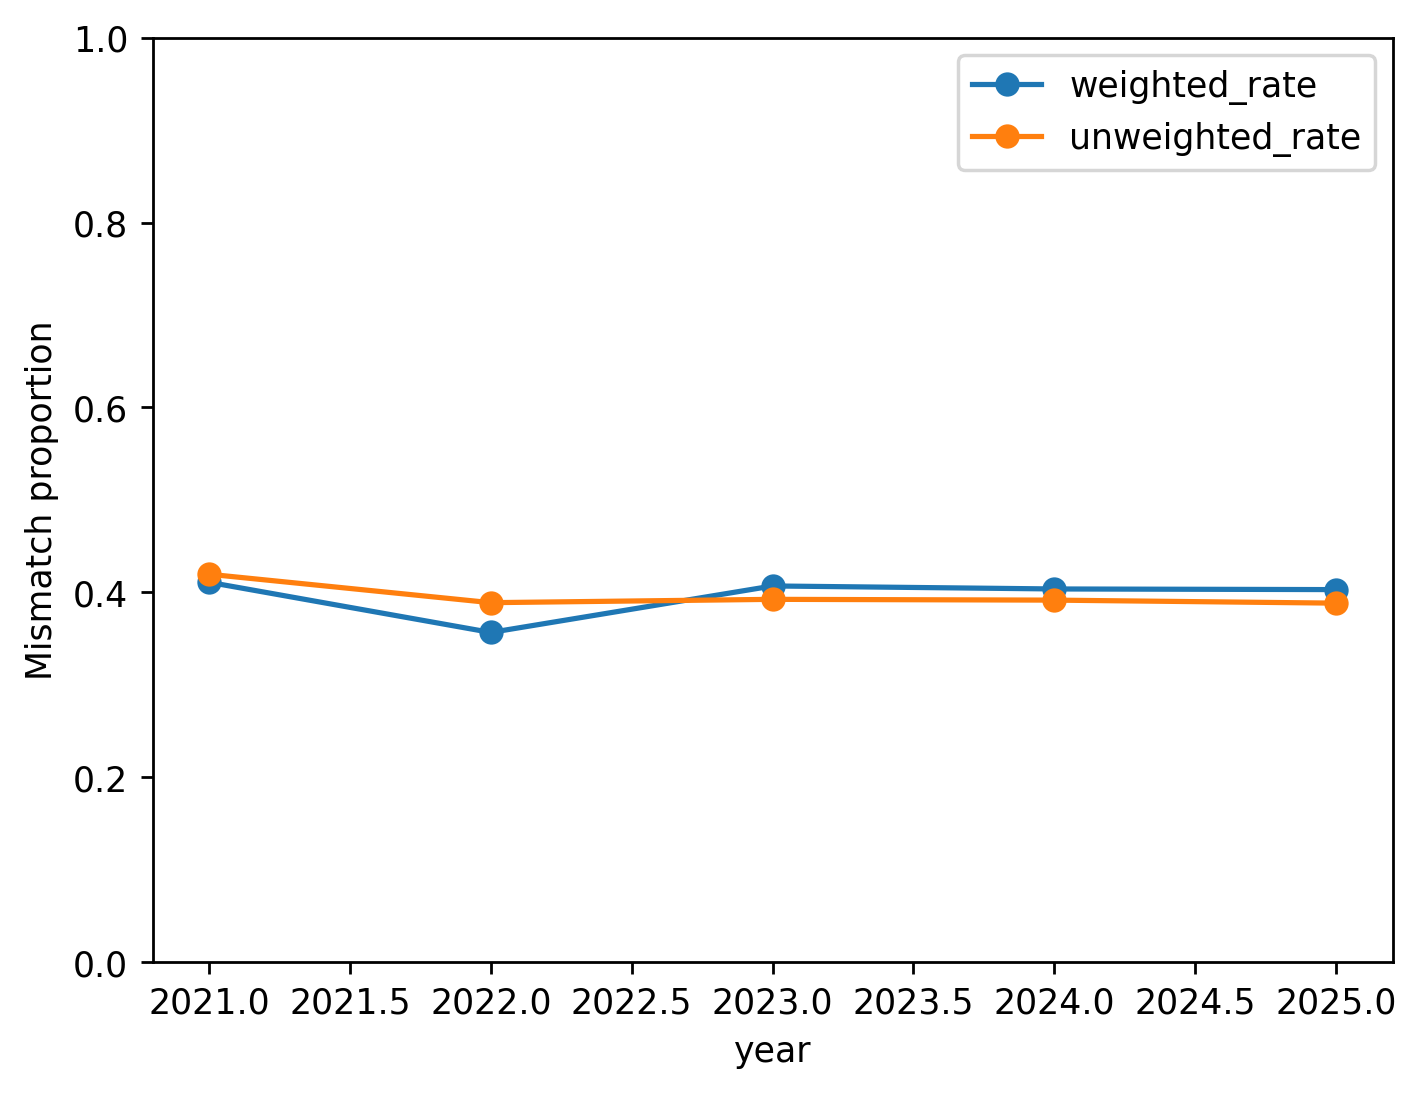
\includegraphics[width=.69\linewidth]{figures/annual_mismatch.png}\caption{Annual weighted and unweighted mismatch among evaluable employed STEM graduates. Source: ENEMDU, project calculations.}\label{fig:annual}\end{figure}

\begin{table}[htbp]\caption{Weighted mismatch by STEM field and sex, 2025. Intervals are approximate 95\% bootstrap intervals.}\label{tab:domains}\centering\small\begin{tabularx}{\linewidth}{Xrrr}\toprule Group & Records & Rate (\%) & Interval (\%)\\\midrule
Natural sciences, mathematics and statistics &442&52.24&43.60--61.42\\
ICT &1082&51.18&41.24--61.28\\
Engineering, industry and construction &3577&34.82&31.11--39.13\\
Men &3769&34.89&31.37--38.64\\
Women &1332&53.67&44.89--61.28\\\bottomrule\end{tabularx}\end{table}
Table~\ref{tab:domains} shows differences by field and sex. Women had a higher weighted mismatch estimate than men in each of the five years. In 2025 the difference was 18.78 percentage points. Age-specific estimates varied, with wide intervals for the youngest and oldest groups. These are descriptive comparisons, not adjusted effects or formal tests of differences.

\subsection{Income and employment conditions}
In 2025 median nominal labour income was USD 898 for compatible records and USD 663 for mismatched records, a difference of USD 235. Adequate employment was more frequent among compatible records, whereas underemployment was more frequent among mismatched records (Table~\ref{tab:income}). The median income ordering was consistent across all five years; mean income was not, as in 2022 the mismatched group had a slightly higher weighted mean. Income was missing or excluded in 72 compatible and 169 mismatched records in 2025, so the income comparison is conditional on retained income responses. Among occupations with at least 50 mismatched records, the leading categories included shop sales assistants (8.34\%) and shopkeepers (6.74\%), weighted shares rather than population counts.
\begin{table}[htbp]\caption{Weighted income and employment conditions in 2025. Income is nominal USD; employment rates use valid activity records.}\label{tab:income}\centering\small\begin{tabular}{lrr}\toprule Indicator & Compatible & Mismatch\\\midrule Records &3121&1980\\ Retained income records &3049&1811\\ Mean income (USD)&1087.65&862.80\\ Median income (USD)&898&663\\ Adequate employment (\%)&82.49&61.36\\ Underemployment (\%)&9.73&18.58\\\bottomrule\end{tabular}\end{table}

\subsection{Predictive performance}
Table~\ref{tab:models} reports weighted 2025 results at the F1 threshold selected in 2024. All fitted classifiers improved AP and ROC-AUC relative to the constant baseline. Logistic regression had the highest ROC-AUC and lowest Brier score; Random Forest had the highest balanced accuracy and specificity, and XGBoost the highest AP and F1. The constant classifier predicts all records as positive at its selected threshold, explaining its high recall and comparable F1. The modest precision and specificity indicate substantial false-positive rates, particularly for logistic regression and XGBoost.
\begin{table}[htbp]\caption{Weighted test performance, 2025, after calibration and validation-based threshold selection.}\label{tab:models}\centering\small\begin{tabular}{lrrrr}\toprule Metric & Constant & LR & RF & XGB\\\midrule ROC-AUC &.5000&.6522&.6434&.6381\\ AP &.4028&.5658&.5579&.5673\\ Precision &.4028&.4142&.4792&.4315\\ Recall &1.0000&.9236&.6974&.8880\\ Specificity &.0000&.1188&.4887&.2108\\ F1 &.5743&.5719&.5681&.5808\\ Balanced accuracy &.5000&.5212&.5931&.5494\\ Brier &.2407&.2233&.2259&.2253\\\bottomrule\end{tabular}\end{table}
\begin{figure}[htbp]\centering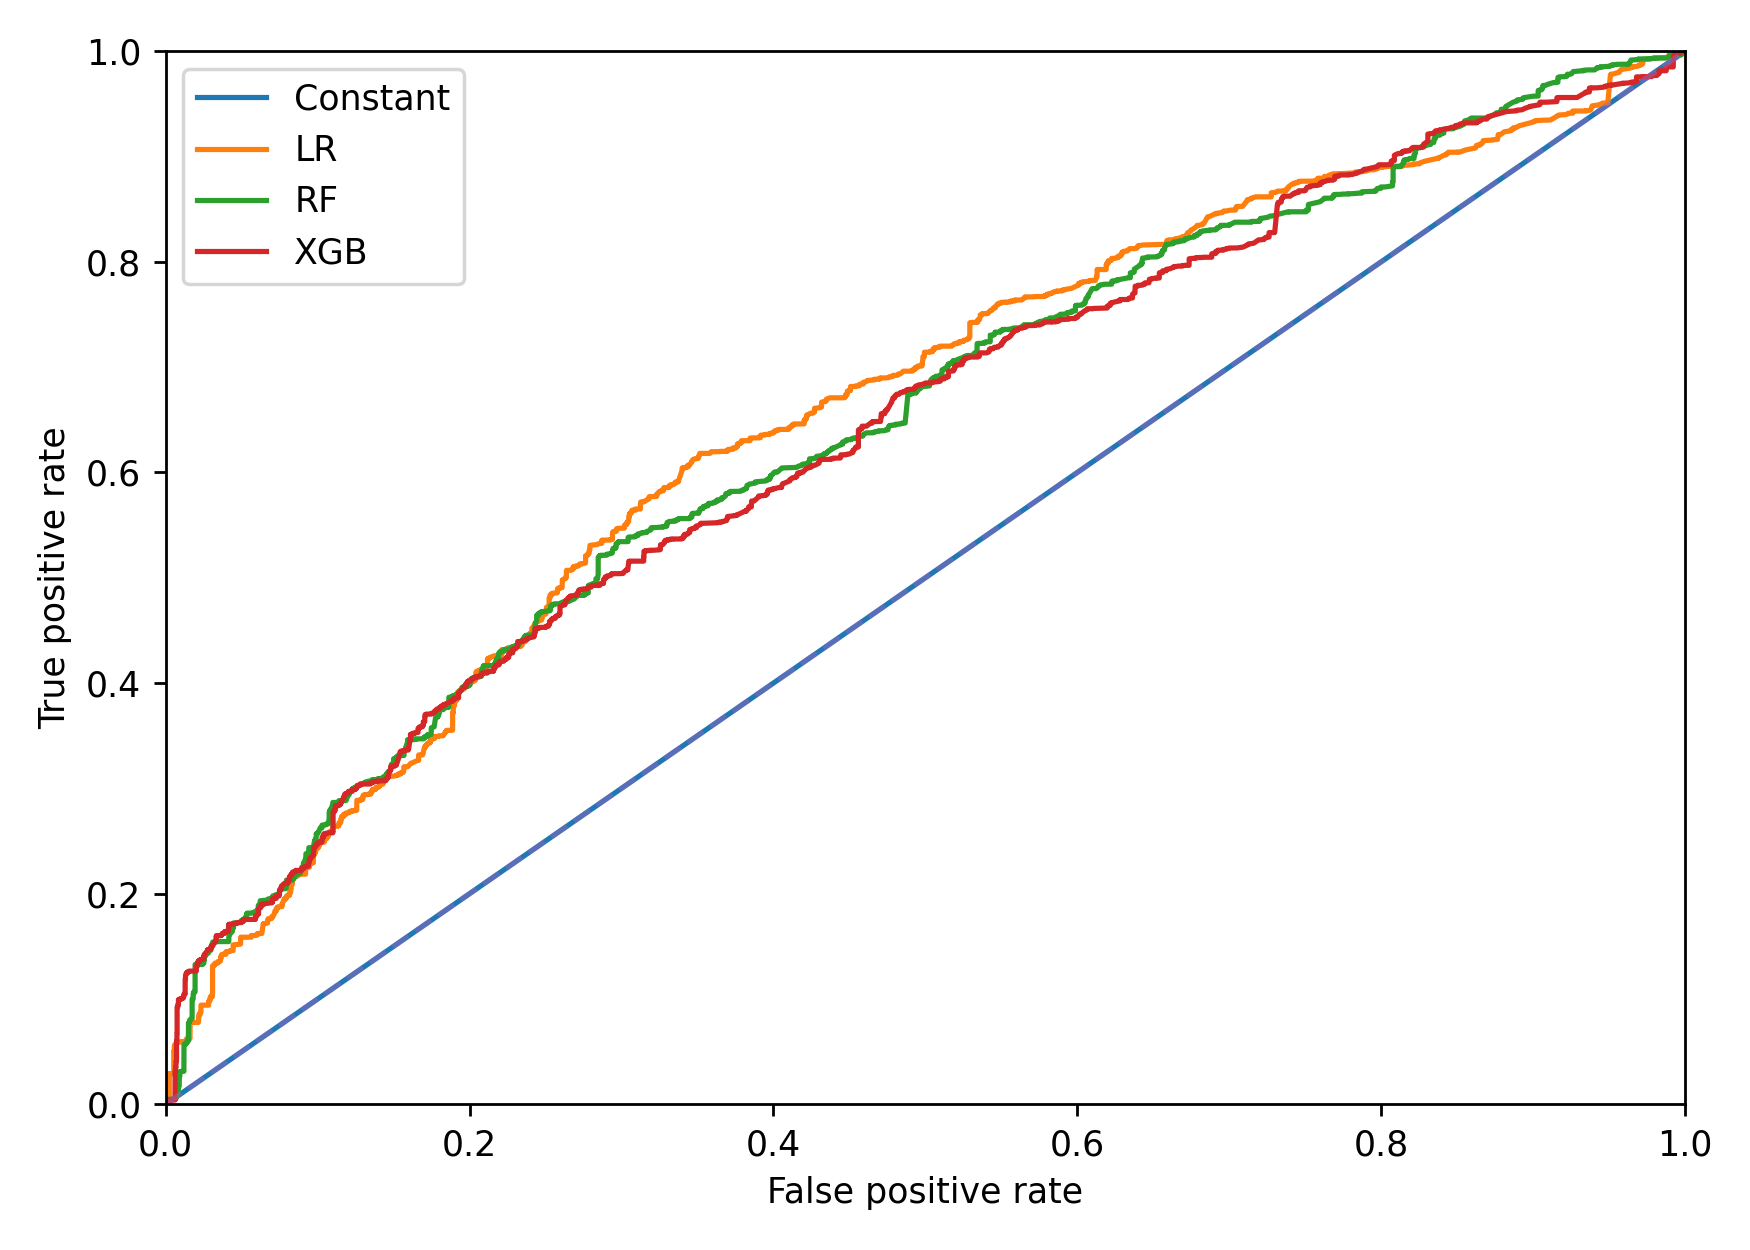
\includegraphics[width=.49\linewidth]{figures/roc.png}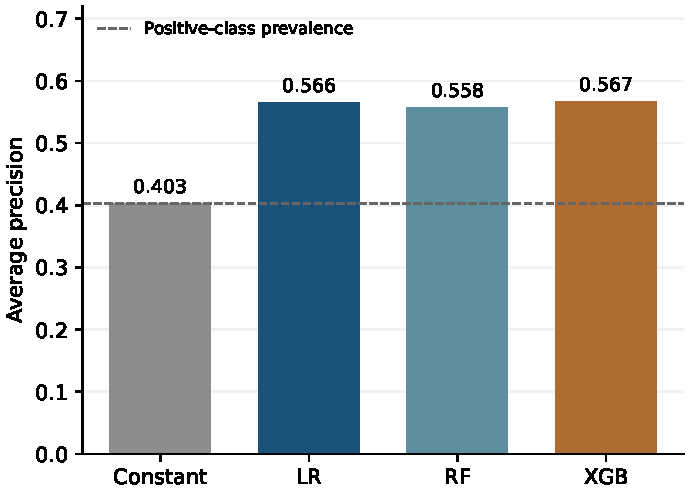
\includegraphics[width=.49\linewidth]{figures/ap_comparison.pdf}\caption{Weighted ROC curves (left) and average precision scores (right) for 2025. The dashed horizontal line denotes positive-class prevalence.}\label{fig:curves}\end{figure}
The paired bootstrap ROC-AUC differences between LR and RF ($-0.0214$ to $0.0373$), LR and XGB ($-0.0136$ to $0.0440$), and RF and XGB ($-0.0176$ to $0.0247$) all included zero. Thus the ordering is descriptive rather than evidence of a clear superiority among fitted models.

\subsection{Interpretation and sensitivity}
Permutation importance identified sex, STEM field and province among the leading predictors in all three models (Figure~\ref{fig:importance}). The leading AP decreases for LR were sex (0.0755), field (0.0365) and province (0.0309); for RF, field (0.0536), sex (0.0411) and province (0.0301); for XGB, field (0.0681), province (0.0481) and sex (0.0417). SHAP was generated for RF but not for XGB due to a software conversion error; the comparable interpretation uses permutation importance.
\begin{figure}[htbp]\centering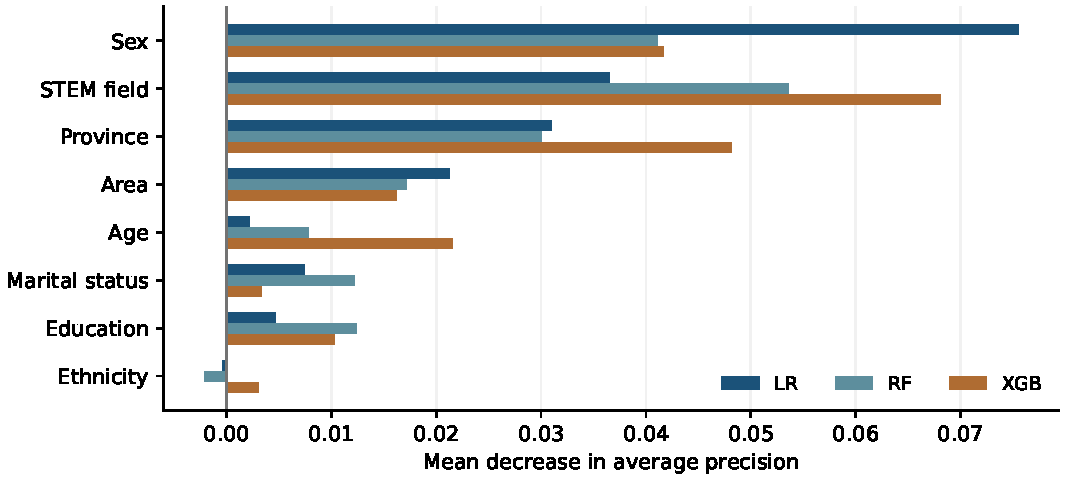
\includegraphics[width=.9\linewidth]{figures/importance_comparison.pdf}\caption{Permutation importance by classifier (mean decrease in AP).}\label{fig:importance}\end{figure}
\begin{table}[htbp]\caption{Weighted ROC-AUC in 2025 under sensitivity scenarios.}\label{tab:sens}\centering\small\begin{tabular}{lrrr}\toprule Scenario & LR & RF & XGB\\\midrule Main &.6522&.6434&.6381\\ Excluding 2021 &.6495&.6383&.6447\\ Without field &.6365&.6151&.6154\\ Unweighted training &.6616&.6476&.6638\\ Candidate household purge &.6502&.6355&.6399\\\bottomrule\end{tabular}\end{table}
Excluding 2021 changed discrimination only modestly. Removing the field reduced ROC-AUC across the three models; unweighted training increased it in the observed test. The candidate household purge reduced training and validation to 12,303 and 3589 records, respectively, while leaving the test unchanged. Performance remained broadly similar (Table~\ref{tab:sens}); this does not establish individual independence. No alternative normative correspondence was evaluated.
